% !Mode:: "TeX:UTF-8"
%!TEX program  = xelatex

\documentclass[bwprint]{gmcmthesis}

\title{对恐怖袭击事件记录数据的量化分析}
\baominghao{18107050029} %参赛队号
\schoolname{西安石油大学}%学校名称
\membera{张鑫} %队员A
\memberb{任萌} %队员B
\memberc{成怡瑶} %队员C
\begin{document}

 %生成标题
 \maketitle

 %填写摘要
\begin{abstract}



%本模板是为全国研究生数学建模竞赛编写的 \LaTeX{} 模板, 旨在让大家专注于
%论文的内容写作, 而不用花费过多精力在格式的定制和调整上. 本手册是相应的参考, 其
%中提供了一些环境和命令可以让模板的使用更为方便. 同时需要注意, 使用者需要有一
%定的 \LaTeX{} 的使用经验, 至少要会使用 ctex 宏包的一些功能, 比如调节字距或修改字体
%大小等等.
%
%
%另外, 欢迎大家购买我们是视频教程,点击\href{https://item.taobao.com/item.htm?spm=a1z10.1-c.w4004-3473795048.4.ThFQCG&id=43823508044}{\fbox{这里}}。
%
%欢迎大家到QQ群里沟通交流:91940767.

%\uwave{关注我们的微信公众号}:

%\centerline{\includegraphics[width=5cm]{gongzhonghao}}


\keywords{恐怖袭击\quad  量化分析\quad   数据可视化\quad  关联规则分析}
\end{abstract}

\pagestyle{plain}

%目录 不推荐加
\tableofcontents


\newpage
\section{问题重述}

\subsection{引言}

恐怖袭击是指极端分子或组织人为制造的、
针对但不仅限于平民及民用设施的、
不符合国际道义的攻击行为,
它不仅具有极大的杀伤力,
能直接造成巨大的人员伤亡和财产损失,
而且还给人们带来巨大的心理压力,
造成社会一定程度的动荡不安,
妨碍正常的工作与生活秩序,
进而极大的阻碍经济的发展。

恐怖主义是人类的共同威胁,
打击恐怖主义是每个国家应该承担的责任。
对恐怖袭击事件相关数据的深入分析有助于加深人们对恐怖主义的认识,
为反恐防恐提供有价值的信息支持。

全球恐怖主义数据库(GTD)中记录了1998-2017年世界上发生的恐怖袭击事件。
数据显示恐怖袭击事件在全球一直发生着并成为全球的不稳定因素,
也有许多国家和地区采取了一系列政策。
但是恐怖袭击是一种突发事件,
其不确定性将对今后事件态势的发展的预估造成很大的影响。
因此,
如何表达数据本身及其包含的不确定性,
成为恐怖袭击数据分析中的重要问题。

\subsection{研究问题}

已知数据变量总共九类:
GTD的标志号和日期、
事件信息、
事件发生的地点、
攻击信息、
武器信息、
目标/受害者信息、
凶手信息、
伤亡和后果、
附加信息和来源。
通过这些信息来对恐怖袭击事件的发生进行深入分析,
从而对反恐防恐提供有价值的信息支持。

\subsubsection{任务一:依据危害性对恐怖袭击事件分级}

对灾难性事件比如地震、交通事故、气象灾害等等进行分级是社会管理中的重要工作。
通常的分级一般采用主观方法,
由权威组织或部门选择若干个主要指标,
强制规定分级标准,
如我国《道路交通事故处理办法》第六条规定的交通事故等级划分标准,
主要按照人员伤亡和经济损失程度划分。
但恐怖袭击事件的危害性不仅取决于人员伤亡和经济损失这两个方面,
还与发生的时机、地域、针对的对象等等诸多因素有关,
因而采用上述分级方法难以
形成统一标准。
依据GTD数据库中的有关信息,
结合现代信息处理技术,
借助数学建模方法建立基于数据分析的量化分级模型,
将GTD中给出的事件按危害程度从高到低分为一至五级,
列出近二十年来危害程度最高的十大恐怖袭击事件,
并给出表1中事件的分级。


\begin{table}
\centering
\caption{典型事件危害级别}
\begin{tabular}{|c|c|}
  \hline
  % after \\: \hline or \cline{col1-col2} \cline{col3-col4} ...
  事件编号 & 危害级别 \\
  \hline
  200108110012 &   \\
  \hline
  200511180002 &   \\
  \hline
  200901170021 &   \\
  \hline
  201402110015 &   \\
  \hline
  201405010071 &   \\
  \hline
  201411070002 &   \\
  \hline
  201412160041 &   \\
  \hline
  201508010015 &   \\
  \hline
  201705080012 &   \\
  \hline
\end{tabular}
\end{table}


\subsubsection{任务二:依据事件特征发现恐怖袭击事件制造者}

GTD数据库中有多起恐怖袭击事件尚未确定作案者。
如果将可能是同一个恐怖组织或个人在不同时间、
不同地点多次作案的若干案件串联起来统一组织侦査,
有助于提高破案效率,
有利于尽早发现新生或者隐藏的恐怖分子。请你们针对在
2015、2016 年度发生的、尚未有组织或个人宣称负责的恐怖袭击事件,
运用数学建模方法寻找上述可能性,
即将可能是同一个恐怖组织或个人在不同时间、不同地点多次作案的若干案件归为一类,
对应的未知作案组织或个人标记不同的代号,
并按该组织或个人的危害性从大到小选出其中的前5个,
记为1号-5号。
再对表2列出的恐袭事件,
按嫌疑程度对5个嫌疑人排序,
并将结果填入下表
(表中样例的意思是:
对事件编号为XX的事件,
3号的嫌疑最大,其次是4号,
最后是5号),
如果认为某嫌疑人关系不大,
也可以保留空格。

\begin{table}
\centering
\caption{恐怖分子关于典型事件的嫌疑度}
\begin{tabular}{|c|c|c|c|c|c|}
  \hline
         & 1号嫌疑人 & 2号嫌疑人 & 3号嫌疑人 & 4号嫌疑人 & 5号嫌疑人 \\
  \hline
  样例XX       &  &  &  &  &  \\
  \hline
  201701090031 &  &  &  &  &  \\
  \hline
  201702210037 &  &  &  &  &  \\
  \hline
  201703120023 &  &  &  &  &  \\
  \hline
  201705050009 &  &  &  &  &  \\
  \hline
  201705050010 &  &  &  &  &  \\
  \hline
  201707010028 &  &  &  &  &  \\
  \hline
  201707020006 &  &  &  &  &  \\
  \hline
  201708110018 &  &  &  &  &  \\
  \hline
  201711010006 &  &  &  &  &  \\
  \hline
  201712010003 &  &  &  &  &  \\
  \hline
\end{tabular}
\end{table}


\subsubsection{任务三:对未来反恐态势的分析}

对未来反恐态势的分析评估有助于提高反恐斗争的针对性和效率。
依据GTD数据库中的内容并结合因特网上的有关信息,
建立适当的数学模型,
研究近三年来恐怖袭击事件发生的主要原因、时空特性、蔓延特性、级别分布等规律,
进而分析研判下一年全球或某些重点地区的反恐态势,
用图/表给出你们的研究结果,
提出你们对反恐斗争的见解和建议。

\subsubsection{任务四:数据的进一步利用}

数据一还可以发挥哪些作用


\section{模型的假设}

\begin{enumerate}
  \item 数据预处理,假设某些空值属性为0;
  \item 任务一:利用机器学习聚类算法对GTD数据库中的feature进行聚类分析;
  \item 任务二:通过关联规则分析得出结果;
  \item 任务三:利用机器学习预测算法对未来反恐态势进行分析。
\end{enumerate}

\section{符号说明}

\begin{tabular}{cc}
 \hline
 \makebox[0.4\textwidth][c]{符号}	&  \makebox[0.5\textwidth][c]{意义} \\ \hline
 D	    & 木条宽度(cm) \\ \hline
 L	    & 木板长度(cm)  \\ \hline
 W	    & 木板宽度(cm)  \\ \hline
 N	    & 第n根木条  \\ \hline
 T	    & 木条根数  \\ \hline
 H	    & 桌子高度(cm)  \\ \hline
 R	    & 桌子半径(cm)  \\ \hline
 R	    & 桌子直径(cm)  \\ \hline
\end{tabular}

\section{问题分析}

在做任务分析之前,
我们看到了GTD数据库中共有114183个样本数据,
109个变量,
其中记录了1998~2017年发生的恐怖袭击的相关信息,
变量总共包含九类:
GTD的标志号和日期、
事件信息、
事件发生的地点、
攻击信息、
武器信息、
目标/受害者信息、
凶手信息、
伤亡和后果。

针对上面数据,
我们首先对恐怖袭击事件发生的时间,
地点(地区和国家),
死亡人数,财产损失,袭击类型,武器类型,袭击目标进行了可视化分析。
通过上面可视化分析可以得到下面的结论。


\subsection{任务一分析}

针对任务一,
其中,
恐怖袭击事件的危害性不仅仅取决于人员伤亡和经济损失两方面,
\cite{贺怀清2012恐怖袭击事件不确定性度量及可视分析}
中将时间、地域性、袭击方式和针对目标作为恐怖袭击事件的危害性度量标准。
其中包含变量年(Year)、
月(Month)、
日(Day)、
国家(Country)、
地区(Region)、
袭击类型(Attack)、
袭击目标(Targ)、
袭击目标和国籍(Natlty)、
武器类型(Weap)、
伤亡人数(Nkill)。
\cite{李国辉2014全球恐怖袭击时空演变及风险分析研究}
中讲到将恐怖袭击的影响因素分为直接影响和间接影响,
其中直接影响包括人员伤亡和经济损失,
这些和恐怖分子采用的武器类型、袭击方式和袭击目标是紧密相关的。
间接影响包括对社会秩序的影响,
这可能是与社会民主制度、政治参与度等有关。
同时,恐怖袭击还与地理空间属性有关。


\subsection{任务二分析}
题目要求从折叠桌的稳固性好、加工方便、用材最少三个角度,确定设计加工参数。我们可以从应力、支撑面积考虑稳固性,从开槽长度考虑加工方便,从木板长度考虑用材最少。而它们之间又是相互制约,我们需要确定最优设计加工参数,可以建立非线性规划模型,用lingo软件来求解最优设计加工参数(平板尺寸、钢筋位置、开槽长度等),这里以合力的方向(斜向上)与最长木条(桌腿)的夹角方向最小为目标函数,以木条所承受应力小于木条的许用应力、支撑面积大于桌面面积、木条的开槽长度小于木条本身长为约束条件。
\begin{figure}[!h]
\centering
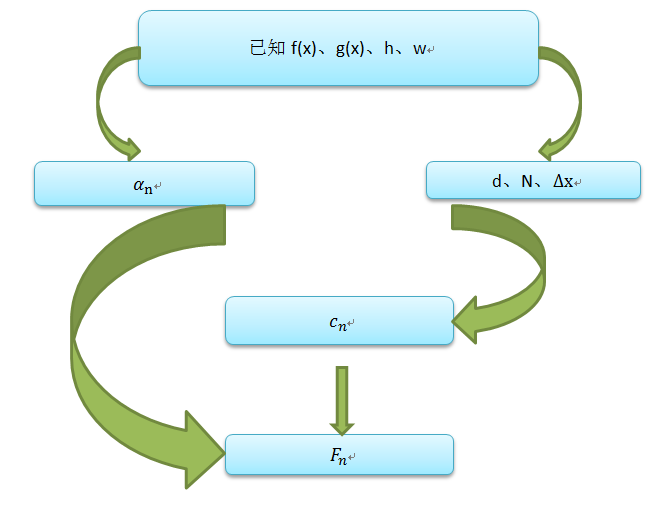
\includegraphics[width=.7\textwidth]{1.png}
\caption{问题三流程图}
\end{figure}
\subsection{任务三分析}
题目要求制作软件的意思就是客户给定折叠桌高度、桌面边缘线的形状大小和桌脚边缘线的大致形状,将这些信息输入程序就得到客户想要的桌子。我们在求解最优设计加工参数时,自行给定桌面边缘线形状(椭圆、相交圆等),桌脚边缘线形状,折叠桌高度,应用第二问的非线性规划模型,用MATLAB软件绘制折叠桌截面图,得到自己设计的创意平板折叠桌。



%参考文献   手工录入
%\begin{thebibliography}{9}%宽度9
% \bibitem{bib:one} ....
% \bibitem{bib:two} ....
%\end{thebibliography}

%采用bibtex方案
\cite{mittelbach_latex_2004,wright_latex3_2009,beeton_unicode_2008,vieth_experiences_2009}

\bibliographystyle{gmcm}
\bibliography{18107050029}


\newpage
%附录
\appendix
%\setcounter{page}{1} %如果需要可以自行重置页码。
\section{我的 MATLAB 源程序}
\begin{lstlisting}[language=Matlab]%设置不同语言即可。
kk=2;[mdd,ndd]=size(dd);
while ~isempty(V)
[tmpd,j]=min(W(i,V));tmpj=V(j);
for k=2:ndd
[tmp1,jj]=min(dd(1,k)+W(dd(2,k),V));
tmp2=V(jj);tt(k-1,:)=[tmp1,tmp2,jj];
end
tmp=[tmpd,tmpj,j;tt];[tmp3,tmp4]=min(tmp(:,1));
if tmp3==tmpd, ss(1:2,kk)=[i;tmp(tmp4,2)];
else,tmp5=find(ss(:,tmp4)~=0);tmp6=length(tmp5);
if dd(2,tmp4)==ss(tmp6,tmp4)
ss(1:tmp6+1,kk)=[ss(tmp5,tmp4);tmp(tmp4,2)];
else, ss(1:3,kk)=[i;dd(2,tmp4);tmp(tmp4,2)];
end;end
dd=[dd,[tmp3;tmp(tmp4,2)]];V(tmp(tmp4,3))=[];
[mdd,ndd]=size(dd);kk=kk+1;
end; S=ss; D=dd(1,:);


 \end{lstlisting}


\end{document}
